\documentclass{beamer}
\usetheme{Berlin}
\usecolortheme{beaver}
\usepackage{graphicx}


\title{Modulation techniques}
\subtitle{Pulse amplitude modulation, Digital pulse modulation}
\author[Riccardo \and Eren]{Riccardo~Miccini\inst{1} \and Eren~Can~\inst{1}}
\institute[DTU]
{
	\inst{1}
	Technical University of Denmark\\
	Digital Communication
}
\date{\today}
\subject{Digital Communication}


\begin{document}

	\frame{\titlepage}

	\begin{frame}
		\frametitle{Analog Pulse Modulation techniques}
		\begin{itemize}
			\item Sample $ \rightarrow $ Pulse
			\item Pulse properties: amplitude, width, phase/position
			\item Modulation technique for each property: PAM, PWM, PPM
		\end{itemize}
	\end{frame}

	\begin{frame}
		\frametitle{Pulse Amplitude Modulation}
		\begin{itemize}
			\item Sequence of pulses with finite width $ \tau $
			\item Signal level $ \rightarrow $ pulse height
			\item Analog signal sampled at pulse edge: $ m_\delta = m(nT_s)\delta(t - nT_s) $
			\item Holding circuit: $ h(t) = rect(\frac{t - \frac{1}{2}\tau}{\tau}) $
		\end{itemize}
	\end{frame}

	\begin{frame}
		\frametitle{Delta Modulation}
		\begin{itemize}
			\item Delta modulation technique in which the message signal is encoded into a sequence of binary symbols.
			\item It is an analog to digital and digital to analog conversion technique.
			\item  It is the simplest form of DPCM cause the transmitted data are reduced to  a 1-bit
		\end{itemize}
	\end{frame}
	
	\begin{frame}
	\frametitle{Explaining the functions and Figures}
	\begin{itemize}
	\item The input that pulse modulator need is: $ d(t)= m(t)-m_s(t) $
    	\item $m(t)$ is the message signal and and $m_s(t)$ is the reference waveform.
	\item $d(t)$ is  hard-limited and it will be multiplied by the pulse generator. So result will be: $x_c(t)$=$\Delta(nT_s)*\delta(t-nT_s)$
	\item Also reference signal will generate by integrating $ x_c(t)$ . Result will be : $m_s(t)$= $\Delta(nT_s)*\int_{}^{t}\delta(\alpha - nT_s)d\alpha $
	\item Demodulation of DM is accomplished by integrating $X_c(t)$ to form stairstep approximation $m_s(t)$
	\end{itemize}
         \end{frame}
         
         \begin{frame}
         \frametitle{Figure}
         \end{frame}
         
         \begin{frame}
         \frametitle{Pulse-Code Modulation}
         \begin{itemize}
         \item The generation of PCM is a three-step process. First, $m_t$ gets sampled, secondly it gets quantinized and encoder.
         \item In PCM,quantized level is transmitted data instead of sample value.
         \item A binary "one" is represented as a pulse, and a binary "zero" represented as pulse.
         \item For the binary requirements, of a PCM system,suppose that q 	quantization levels following formula  will be used: $q=2^n$ where n is the word length, integer. For this case, $n=log_2*q$ ,binary pulses must be transmitted for each sample of the message signal.
         \end {itemize}
         \end{frame}
         
         \begin{frame}
         \frametitle{Time- Division Multiplexing}
         \begin{itemize}
         \item Time-Division multiplexing is best understood by considering the figure below
         \end{itemize}
         \begin{figure}
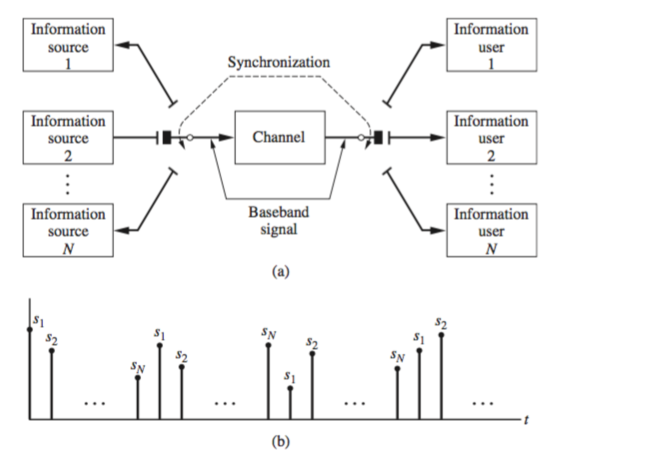
\includegraphics[width=\textwidth,height= 10cm,keepaspectratio]{fig1.png}
  \caption{Investigating TDM.}
  \label{fig:time-divison1}
\end{figure}
\begin{itemize}
\item	 At the output,
\end{itemize}
         \end{frame}

\end{document}
